\section{Code Footprint \& Security}
Compiling unikernel applications produces a single artifact, which is the machine image. That image can be booted directly with very little configuration. Many unikernels can also be compiled to a single binary that runs on the host operating system without a hypervisor. Table \ref{tab:sizes} shows the sizes of produced images for different targets. The Docker is a different case. It is just the binary image copied inside the Ubuntu container. It's there for representing environments where unikernels and containers coexist. When compiled for Xen, MirageOS also produces a configuration file to pass to hypervisor. That file is only couple of lines long and is not mandatory. The configuration on it can be passed directly through flags. The only changing part of the file is name of the image. Other parameters are always the same for different applications if they have the same requests from the hypervisor. That's why this file is omitted and its configuration is hardcoded directly into the Xen command. That additional file is also responsible for networking, if it exists, so those options have to be passed through the deployment template.


\begin{table}[htpb]
  
  \centering
  \begin{tabular}{ |c|c| }
    \toprule
      Hypervisor & Size \\
    \midrule
    Docker* & 69.4 MB \\
     
      \hline
      Binary & 4.7 MB \\
    \hline
    Xen &  3.3 MB\\
    \hline
    Virtio & 2.4 MB \\
    \hline
      Hvt & 2.3 MB\\
    \bottomrule
  \end{tabular}
  \caption[Image Sizes]{Image sizes}\label{tab:sizes}
\end{table}


It's clear in the table that compiling unikernel for a hypervisor has a smaller code footprint than other options. Virtio and Hvt have smaller artifacts than Xen. Although, it should be noted that running those images requires Solo5 on top of Qemu or KVM to be installed on the system. For Xen image, only the hypervisor is enough. Nevertheless, when we compare the sizes of those artifacts with traditional operating system images, as they are also operating systems, it's easy to see that they are much more smaller, albeit with much less functionality, which is desired in that case.

Unikernels tell a much more different story in application security than operating systems or containers. Unikernel only has the code required by the application and that greatly reduces attack surface. As once said by Meireles  \textit{".. while you can sometimes attack what you can't see, you can't attack what is not there."} \cite{mailing-list}. An application running on a VM can be affected by the vulnerabilities of the underlying operating system on top of its own possible vulnerabilities. A Dockerized application can be affected by the vulnerabilities in the Docker daemon. Some of Docker related vulnerabilities can be found in \cite{CVE-2019-14271-details}, \cite{CVE-2018-9862-details}, \cite{CVE-2018-8115-details}, \cite{CVE-2018-11757-details}, \cite{CVE-2019-5736-details}. In a unikernel environment, the only parts that are suitable for attack are the hypervisor itself, and the application. Because there are no other open ports possibly compromising the system, the application itself can be tested for weaknesses in a much more known, secure and controlled environment.

Unikernels are also single address space applications. Figure \ref{fig:normal} shows how a traditional application operates and how isolation of address spaces handled in OS. There are two different address spaces and compromising kernel space is enough to compromise all the applications running on top of it. In figure \ref{fig:uni} we see how a unikernel application handles its own address space. To compromise that application, there is no other way than to attack the application itself. This also makes unikernel application faster to operate, because there is no process management layer as a unikernel only has a single process, which is itself. Duncan et al. concludes in \cite{Duncan2017} that \textit{"unikernel approach might offer a better solution"} to key security issues.
\begin{figure}[htbp]
    \centering
    \subfloat[Normal application Stack]{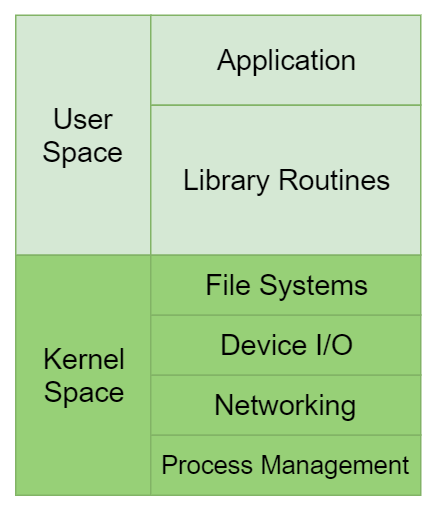
\includegraphics[width=0.4\textwidth]{figures/normal_application_stack.png}\label{fig:normal}}
    \hfill
    \subfloat[Unikernel application Stack]{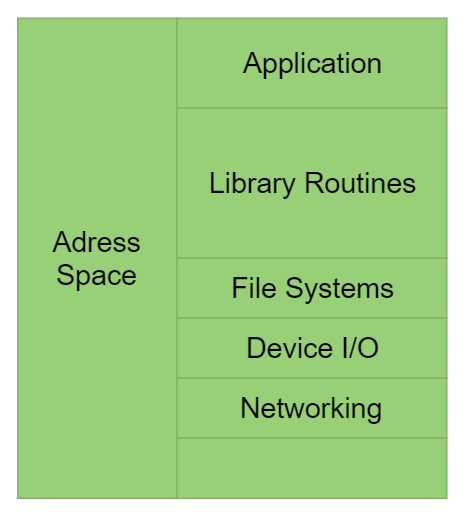
\includegraphics[width=0.4\textwidth]{figures/unikernel_application_stack.png}\label{fig:uni}}
    \caption{Address space security}\label{fig:single-space}
  \end{figure}

